% ============================================================================
%  Four worked examples: convergence rates as transfer-matrix contractions
%
%  A short, self-contained companion note. No bibliography file needed
%  (key references are in footnotes); compile with:  pdflatex examples.tex
%  Figures are produced by code/run_all.py and live in figures/.
% ============================================================================
\documentclass[11pt]{article}

\usepackage[a4paper, margin=1in]{geometry}
\usepackage{amsmath, amssymb, mathtools, bm}
\usepackage{graphicx}
\usepackage{booktabs}
\usepackage[dvipsnames]{xcolor}
\usepackage{enumitem}
\usepackage[colorlinks=true, linkcolor=NavyBlue!70!black,
            urlcolor=BrickRed!70!black]{hyperref}

% --- light, uniform layout helpers ------------------------------------------
\newcommand{\R}{\mathbb{R}}
\newcommand{\tr}{\operatorname{tr}}
\newcommand{\rank}{\operatorname{rank}}
\newcommand{\eqdef}{\coloneqq}
\newcommand{\one}{\mathbf 1}
\newcommand{\spec}{\rho}                 % spectral radius / Perron eigenvalue
% run-in field labels used identically in every example:
\newcommand{\F}[1]{\smallskip\noindent\textbf{\textsf{#1.}}\hspace{0.4em}}

\setlist{leftmargin=1.5em}

\title{\bf Four convergence rates, computed as transfer--matrix contractions}
\date{\today}

\begin{document}
\maketitle
\vspace{-1.5em}

\begin{abstract}
\noindent
A great many ``rates'' in analysis, dynamics and combinatorics are the
exponential growth rate of a sum over words,
$Z_L=\sum_{|I|=L}\omega(I)$. Whenever the weight $\omega$ is carried by a
\emph{finite transfer matrix} $T$ -- so that $Z_L=\langle u,T^Lv\rangle$ -- the
rate is simply the top eigenvalue of $T$, and the \emph{speed} at which the naive
ratio $Z_{L+1}/Z_L$ settles is the \emph{spectral gap}. Below are four worked
examples that make this concrete, from the trivial to the genuinely hard. Each
states the object in one line, writes the series and its transfer engine
explicitly, and reports the number we actually computed (code in
\texttt{code/}). The reader who wants only the punchlines can read
Table~\ref{tab:summary} and skip to the figures.
\end{abstract}

% ----------------------------------------------------------------------------
\section*{The one fact behind all four}
% ----------------------------------------------------------------------------
\addcontentsline{toc}{section}{The one fact behind all four}

Fix a finite alphabet, let $\mathcal W_L$ be the admissible words of length $L$,
and let $\omega\ge0$ be multiplicative along a word. The object of interest is
\begin{equation}
\label{eq:template}
   Z_L \;=\; \sum_{I\in\mathcal W_L}\omega(I),
   \qquad\qquad
   \lambda \;=\; \lim_{L\to\infty} Z_L^{\,1/L}
   \quad(\text{the \emph{rate}}),
   \qquad P=\log\lambda.
\end{equation}
Say the family is \emph{transfer-decomposable} if there is a fixed matrix
$T\ge0$ and boundary vectors $u,v$ with
\begin{equation}
\label{eq:transfer}
  \boxed{\,Z_L=\langle u,\,T^{L}\,v\rangle\quad\text{for all }L.\,}
\end{equation}
By Perron--Frobenius, if $T$ is primitive with eigenvalues
$|\lambda_1|>|\lambda_2|\ge\cdots$, then
\begin{equation}
\label{eq:rate-gap}
  \boxed{\;\lambda=\lambda_1=\spec(T),\qquad
  \frac{Z_{L+1}}{Z_L}=\lambda_1\Bigl(1+O(\delta^{L})\Bigr),\qquad
  \delta\eqdef\frac{|\lambda_2|}{\lambda_1}\in[0,1).\;}
\end{equation}
So the rate is an \emph{eigenvalue} (computed once, exactly), and the
``divide out the conjectured rate and watch the ratio go to $1$'' heuristic is
not only correct -- its convergence slope on a log plot \emph{is} the spectral
gap $\delta$. The only question is whether a \emph{finite} $T$ exists:

\begin{center}
\renewcommand{\arraystretch}{1.2}
\begin{tabular}{@{}p{0.46\textwidth}p{0.46\textwidth}@{}}
\toprule
\textbf{Decomposable} (finite $T$ exists) & \textbf{Entangled} (it does not)\\
\midrule
rate $=\spec(T)$, computed exactly; cost grows like the matrix dimension
& no finite $T$; brute-force the $q^L$ words and \emph{fit} the rate\\
Examples 1--3 & Example 4\\
\bottomrule
\end{tabular}
\end{center}

\begin{table}[h]
\centering
\renewcommand{\arraystretch}{1.35}
\small
\begin{tabular}{@{}p{0.5cm}p{3.3cm}p{4.4cm}p{4.6cm}@{}}
\toprule
 & \textbf{Quantity (known value)} & \textbf{Series \& engine} & \textbf{What we computed}\\
\midrule
1 & golden ratio $\varphi=1.61803398875$
  & binary words, no ``$11$''; $T=\bigl(\begin{smallmatrix}1&1\\1&0\end{smallmatrix}\bigr)$
  & ratio $\to\varphi$; error slope $=$ gap $\varphi^{-2}$ (meas.\ $0.381965$)\\
2 & hard-square constant $\kappa=1.50304808$
  & strip width $W$; $\dim T_W=F_{W+2}$
  & $\kappa$ to \textbf{13 digits} at $W=14$\\
3 & $\dim_H E_2=0.5312805062772$
  & Gauss-map operator $\mathcal L_s$
  & \textbf{15 digits} at grid $N=16$; ratio test $\to1$ iff $s=s^\ast$\\
4 & matrix-product rate / affinity dim.
  & $T_I=T_{i_1}\!\cdots T_{i_L}$; graph $K_L$ (no finite $T$)
  & surrogate $=\log\spec(T_1{+}T_2)$; affinity dim $s^\ast\!\approx\!1.089$\\
\bottomrule
\end{tabular}
\caption{The four examples at a glance.}
\label{tab:summary}
\end{table}

% ----------------------------------------------------------------------------
\section{Golden-mean shift --- the cleanest case}
% ----------------------------------------------------------------------------

\F{Compute} The number of binary strings of length $L$ with no two adjacent
$1$s. The growth rate is the golden ratio.

\F{Series} With $\mathcal W_L=\{x\in\{0,1\}^L : x_ix_{i+1}=0\ \forall i\}$ and
$\omega\equiv1$,
\[
   Z_L=\#\mathcal W_L=F_{L+2}\quad(\text{Fibonacci}):\quad
   3,5,8,13,21,34,\dots
\]

\F{Engine \& rate} A word is built one bit at a time, the only memory being the
previous bit, so $Z_L=\one^\top T^L\one$ with the $2\times2$ transfer matrix
\[
   T=\begin{pmatrix}1&1\\1&0\end{pmatrix},
   \qquad
   \lambda_{1,2}=\frac{1\pm\sqrt5}{2},
   \qquad
   \boxed{\;\lambda=\lambda_1=\varphi=\tfrac{1+\sqrt5}{2},\quad
   \delta=\frac{|\lambda_2|}{\lambda_1}=\varphi^{-2}.\;}
\]

\F{Result} $Z_{L+1}/Z_L\to\varphi=1.6180339887\ldots$, and the error
$|Z_{L+1}/Z_L-\varphi|$ falls geometrically with measured per-step factor
$0.381965$ against the predicted gap $\varphi^{-2}=0.381966$
(Figure~\ref{fig:1}). \emph{The slope of the error plot is the spectral gap} --
equation~\eqref{eq:rate-gap} in its purest form.

\begin{figure}[h]
\centering
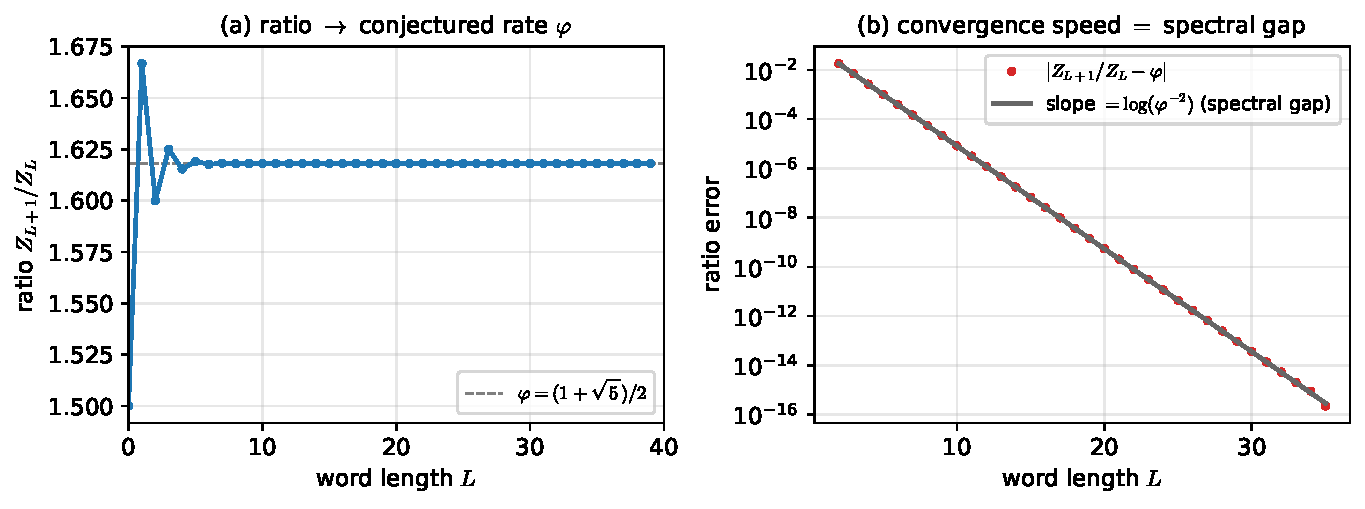
\includegraphics[width=\textwidth]{figures/exp1_golden_mean.pdf}
\caption{Golden-mean shift. (a) the ratio reaches $\varphi$;
(b) the divided-out error decays at exactly the spectral-gap rate $\varphi^{-2}$.}
\label{fig:1}
\end{figure}

% ----------------------------------------------------------------------------
\section{Hard squares on a strip --- width is the cost/accuracy dial}
% ----------------------------------------------------------------------------

\F{Compute} Ways to occupy cells of a $W\times L$ grid with no two occupied
cells edge-adjacent (the hard-core lattice gas). The per-cell growth rate
converges, as $W\to\infty$, to the hard-square constant
$\kappa=1.5030480824753\ldots$\footnote{R.~J.~Baxter, \emph{J.\ Phys.\ A}
(1980); N.~Calkin and H.~Wilf, \emph{SIAM J.\ Discrete Math.}\ (1998).}

\F{Series} $Z_{W,L}=$ number of independent sets of the $W\times L$ grid graph,
summed along the length $L$.

\F{Engine \& rate} Read the grid column by column: the state is the occupied set
of one width-$W$ column, which must itself be an independent set of the path
$P_W$. This gives a transfer matrix $T_W$ with
\[
   \dim T_W=\#\{\text{independent sets of }P_W\}=F_{W+2}\sim\varphi^{\,W},
   \qquad Z_{W,L}=\one^\top T_W^{\,L}\,\one,
\]
\[
   \boxed{\;\kappa=\lim_{W\to\infty}\spec(T_W)^{1/W}
   =\lim_{W\to\infty}\frac{\spec(T_W)}{\spec(T_{W-1})}.\;}
\]
The matrix \emph{dimension} $F_{W+2}\sim\varphi^W$ grows exponentially in the
strip width $W$ --- so $W$ is a dial that buys accuracy at exponential cost.

\F{Result} The incremental ratio $\spec(T_W)/\spec(T_{W-1})$ converges
\emph{geometrically} and already matches $\kappa$ to \textbf{13 digits} at
$W=14$ ($1.503048082\ldots$); see Figure~\ref{fig:2}.

\begin{figure}[h]
\centering
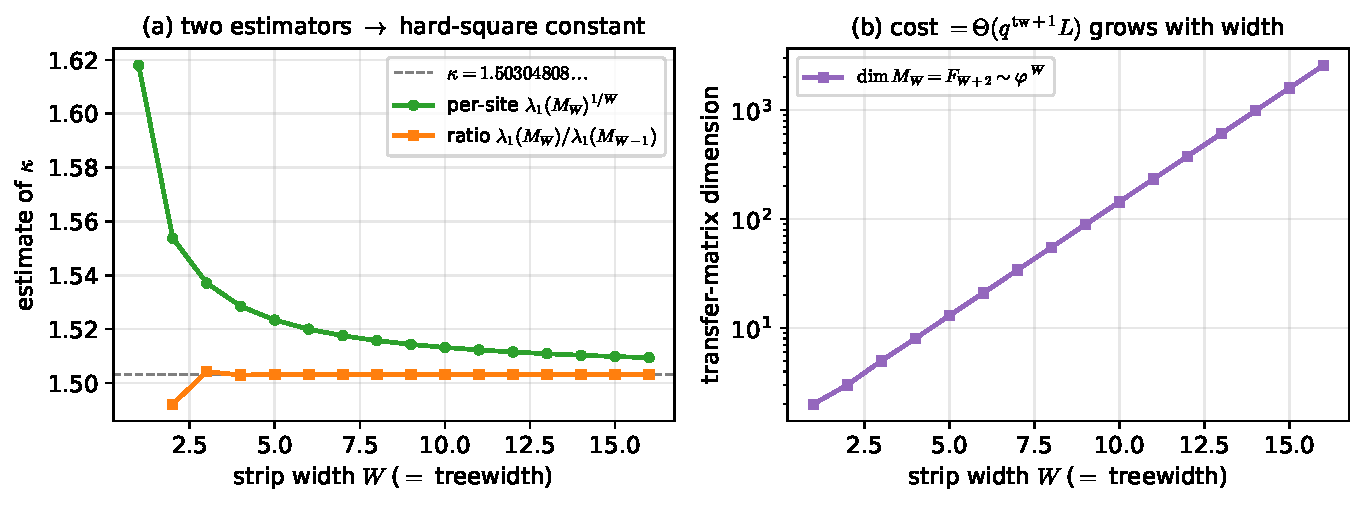
\includegraphics[width=\textwidth]{figures/exp2_hard_squares.pdf}
\caption{Hard squares on a width-$W$ strip. (a) two estimators converge to
$\kappa$ (the ratio estimator geometrically); (b) the transfer-matrix dimension
$F_{W+2}\sim\varphi^W$ --- the cost --- grows with the width.}
\label{fig:2}
\end{figure}

% ----------------------------------------------------------------------------
\section{Continued-fraction set $E_2$ --- a transcendental dimension to 15 digits}
% ----------------------------------------------------------------------------

\F{Compute} The Hausdorff dimension of
$E_2=\{[0;a_1,a_2,\dots]:a_i\in\{1,2\}\}$, the reals whose continued-fraction
digits are all $1$ or $2$. It is a transcendental constant
$s^\ast=0.5312805062772\ldots$\footnote{O.~Jenkinson and M.~Pollicott,
\emph{Adv.\ Math.}\ (2001) and ``\emph{A hundred decimal digits\ldots}''
(2018), the reference value used here.} known only through such computations.

\F{Series} For a word $I=(a_1,\dots,a_L)$ let
$\psi_a(x)=\tfrac1{a+x}$ and $\psi_I=\psi_{a_1}\!\circ\cdots\circ\psi_{a_L}$. The
weight $\omega_I(s)=\sup_x|\psi_I'(x)|^{s}$ is multiplicative along the word
(chain rule), and $Z_L(s)=\sum_{|I|=L}\omega_I(s)$.

\F{Engine \& rate} The infinite Gauss map collapses onto a \emph{fixed} operator
acting on functions on $[0,1]$,
\[
   (\mathcal L_s f)(x)=\sum_{a\in\{1,2\}}(a+x)^{-2s}\,
   f\!\Bigl(\tfrac{1}{a+x}\Bigr),
\]
whose leading eigenvalue $\lambda(s)$ is the rate of $Z_L(s)$. Bowen's equation
gives the dimension as the root where the rate is $1$:
\[
   \boxed{\;s^\ast \text{ is the unique } s \text{ with } \lambda(s)=1.\;}
\]
We discretise $\mathcal L_s$ by Chebyshev collocation on $N{+}1$ nodes
(\emph{independent of word length}) and root-find in $s$.

\F{Result} Two cross-checked routes (Figure~\ref{fig:3}):
\begin{itemize}[itemsep=1pt]
\item \textbf{operator:} at $N=16$ nodes, $s^\ast=0.5312805062772$ --- correct to
\textbf{15 digits}; convergence in $N$ is spectral (each few nodes add several
digits). The operator's gap is $\delta\approx0.31$.
\item \textbf{elementary ratio test:} enumerating all $2^L$ words,
$Z_{L+1}(s)/Z_L(s)\to1$ \emph{exactly when} $s=s^\ast$: at $s^\ast$ the ratio is
$1.000000$, while at $s^\ast\mp0.03$ it locks onto $1.0387$ and $0.9628$. This is
the textbook ``set $s$ to the guess, check the ratio $\to1$'' made rigorous.
\end{itemize}

\begin{figure}[h]
\centering
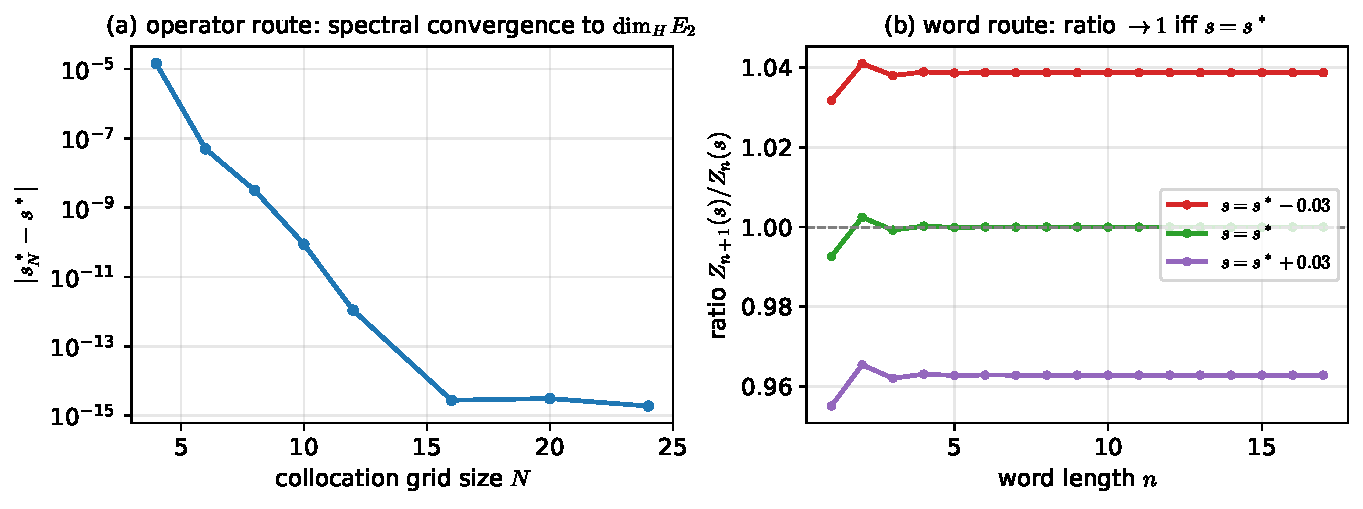
\includegraphics[width=\textwidth]{figures/exp3_continued_fraction.pdf}
\caption{Dimension of $E_2$. (a) spectral convergence of the operator estimate;
(b) the word-enumeration ratio tends to $1$ only at the true dimension.}
\label{fig:3}
\end{figure}

% ----------------------------------------------------------------------------
\section{Matrix products --- the entangled case, and when it collapses}
% ----------------------------------------------------------------------------

\F{Compute} Rates built from products $T_I=T_{i_1}T_{i_2}\cdots T_{i_L}$ of a
fixed set of matrices: the joint spectral radius and Falconer's \emph{affinity
dimension}\footnote{K.~Falconer, \emph{Math.\ Proc.\ Camb.\ Phil.\ Soc.}\
(1988).} of a self-affine set,
\[
   Z_L(s)=\sum_{|I|=L}\varphi^{s}(T_I),
   \qquad
   \varphi^{s}(A)=
   \begin{cases}
     \sigma_1(A)^{s}, & 0\le s\le1,\\[2pt]
     \sigma_1(A)\,\sigma_2(A)^{\,s-1}, & 1\le s\le2,
   \end{cases}
\]
with $\sigma_1\ge\sigma_2$ the singular values. This weight is a \emph{global}
function of the \emph{whole} product, so every index is coupled to every other:
the dependency graph is the complete graph $K_L$, there is \emph{no} finite
transfer matrix, and exact evaluation costs $q^L$. This is the ``everything in
one lump'' case. We use the explicit nonnegative pair
\[
  T_1=\begin{pmatrix}0.50&0.20\\0.10&0.40\end{pmatrix},\qquad
  T_2=\begin{pmatrix}0.30&0.05\\0.25&0.45\end{pmatrix}.
\]

\F{(a) Collapse onto a decomposable surrogate} Replace the operator norm
$\sigma_1=\|\cdot\|$ by the \emph{linear} functional $\tr$. Linearity makes the
weight multiplicative again, and the $K_L$ entanglement collapses to a path:
\[
   \sum_{|I|=L}\tr(T_I)=\tr\!\bigl(S^{L}\bigr),\qquad S=T_1+T_2,
   \qquad(\text{treewidth }1,\ \text{cost }O(L)).
\]
For \emph{nonnegative} matrices Perron--Frobenius forces the norm-rate and this
cheap surrogate to share one limit,
\[
   \boxed{\;\lim_{L\to\infty}\frac1L\log\!\sum_{|I|=L}\|T_I\|
   =\log\spec(T_1+T_2).\;}
\]
Numerically $\log\spec(S)=0.114986731574$ (closed form), and the brute-force
norm-sum over all $2^L$ words drifts onto it (Figure~\ref{fig:4}a). The honest
boundary: for a \emph{signed} pair the cancellation breaks the identity --- our
example gives norm-rate $0.149$ against $\log\spec(S)=-0.153$ --- and one then
needs the projective transfer operator instead of the trace.

\F{(b) Affinity dimension as a pressure root} The affinity dimension is the root
of $P(s)=\lim_L\frac1L\log Z_L(s)=0$. Brute force at $L=18$ gives
$s^\ast\approx1.089$ (Figure~\ref{fig:4}b). The endpoint $s=2$ is a \emph{free
check}: there $\varphi^2=|\det|$ is fully multiplicative, so
$Z_L(2)=(|\det T_1|+|\det T_2|)^L$ in closed form, and brute force reproduces
$\frac1L\log Z_L(2)=-1.195674002$ to every printed digit.

\begin{figure}[h]
\centering
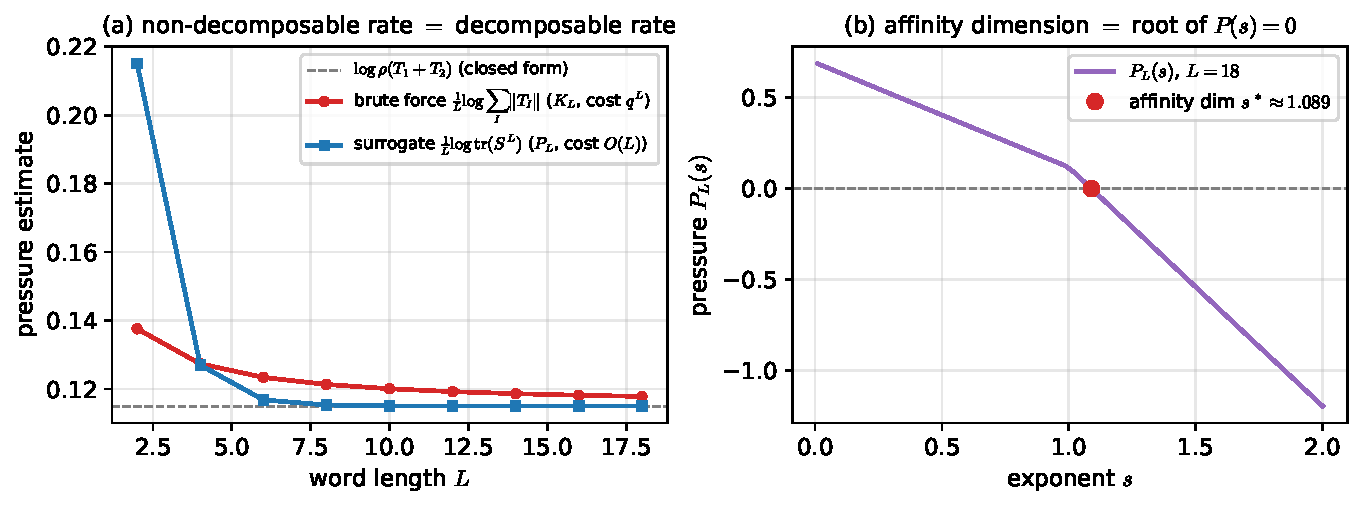
\includegraphics[width=\textwidth]{figures/exp4_matrix_products.pdf}
\caption{Matrix products (entangled, graph $K_L$). (a) the expensive norm-sum
rate and the cheap trace surrogate share the limit $\log\spec(T_1{+}T_2)$ for
nonnegative matrices; (b) the affinity dimension as the root of $P(s)=0$, with
$s=2$ a closed-form validation.}
\label{fig:4}
\end{figure}

\bigskip
\noindent\textit{Reproduce:} \texttt{python3 code/run\_all.py} regenerates every
number and figure above; each script prints the reference constant it matches.

\end{document}
